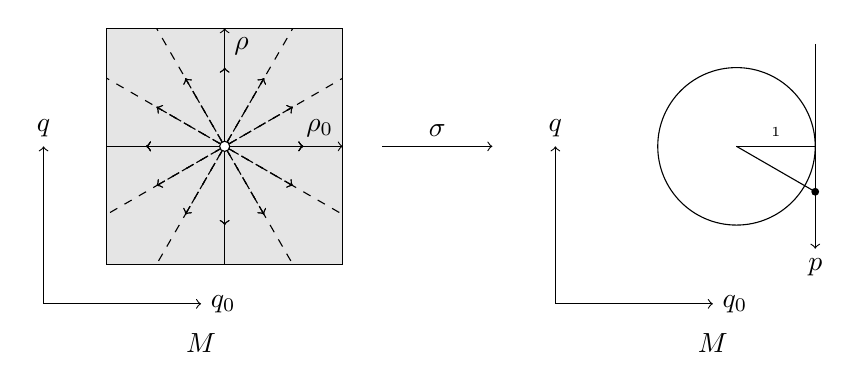
\begin{tikzpicture}
    \draw[->] (0, 0) -- (2, 0) node[anchor=west] {$q_0$};
    \draw[->] (0, 0) -- (0, 2) node[anchor=south] {$q$};
    
    \node (m) at (2.3, 2) {};
    
    \filldraw[draw=black, fill=gray!20] (m) ++(-1.5, -1.5) -- ++(0, 3) -- ++(3, 0) -- ++(0,-3) -- cycle;
    \draw[->] (m) ++(-1.5, 0) -- ++(3, 0) node[anchor=south east] {$\rho_0$};
    \draw[->] (m) ++(0, -1.5) -- ++(0, 3) node[anchor=north west] {$\rho$};
        
    \begin{scope}
        \clip (m) ++(-1.5,-1.5) rectangle ++(3, 3);
        \foreach \i in {0,30,...,180}{
            \draw[<->, dashed] (m) ++({-cos(\i)}, {-sin(\i)}) -- ++({2*cos(\i)}, {2*sin(\i)});
        }
        \foreach \i in {0,30,...,180}{
            \draw[<->, dashed] (m) ++({-cos(\i)}, {-sin(\i)}) -- ++({2*cos(\i)}, {2*sin(\i)});
        }
        \foreach \i in {0,30,...,180}{
            \draw[dashed] (m) ++({-4*cos(\i)}, {-4*sin(\i)}) -- ++({8*cos(\i)}, {8*sin(\i)});
        }
    \end{scope}
    
    \node[circle,draw=black,fill=white,inner sep=1.3pt] at (m) {};
    
    \draw[->] (6.5, 0) -- (8.5, 0) node[anchor=west] {$q_0$};
    \draw[->] (6.5, 0) -- (6.5, 2) node[anchor=south] {$q$};
    
    \node[fill=none] (m2) at (8.8, 2) {};
    
    \draw (m2) circle (1);
    \draw[->] (m2) ++(1, 1.3) -- ++(0, -2.6) node[anchor=north] {$p$} ;
    \draw (m2.center) -- ++(1, -0.577) node[circle,fill=black, inner sep = 1pt] {};
    \draw (m2.center) -- ++(1, 0) node[pos=0.5,anchor=south] {\tiny{1}};
    %\draw[->] (m) ++(-1.5, 0) -- ++(3, 0) node[anchor=west] {$\rho_0$};
    %\draw[->] (m) ++(0, -1.5) -- ++(0, 3) node[anchor=south] {$\rho$};
    
    \draw[->] (4.3, 2) -- (5.7, 2) node[pos=0.5,anchor=south] {$\sigma$};
     
    \node at (2, -0.5) {$\ctzbundle{M}$};
    \node at (8.5, -0.5) {$\pctbundle{M}$};
\end{tikzpicture}
